\documentclass{standalone}
\usepackage{tikz}
\usetikzlibrary{patterns, positioning}


\begin{document}
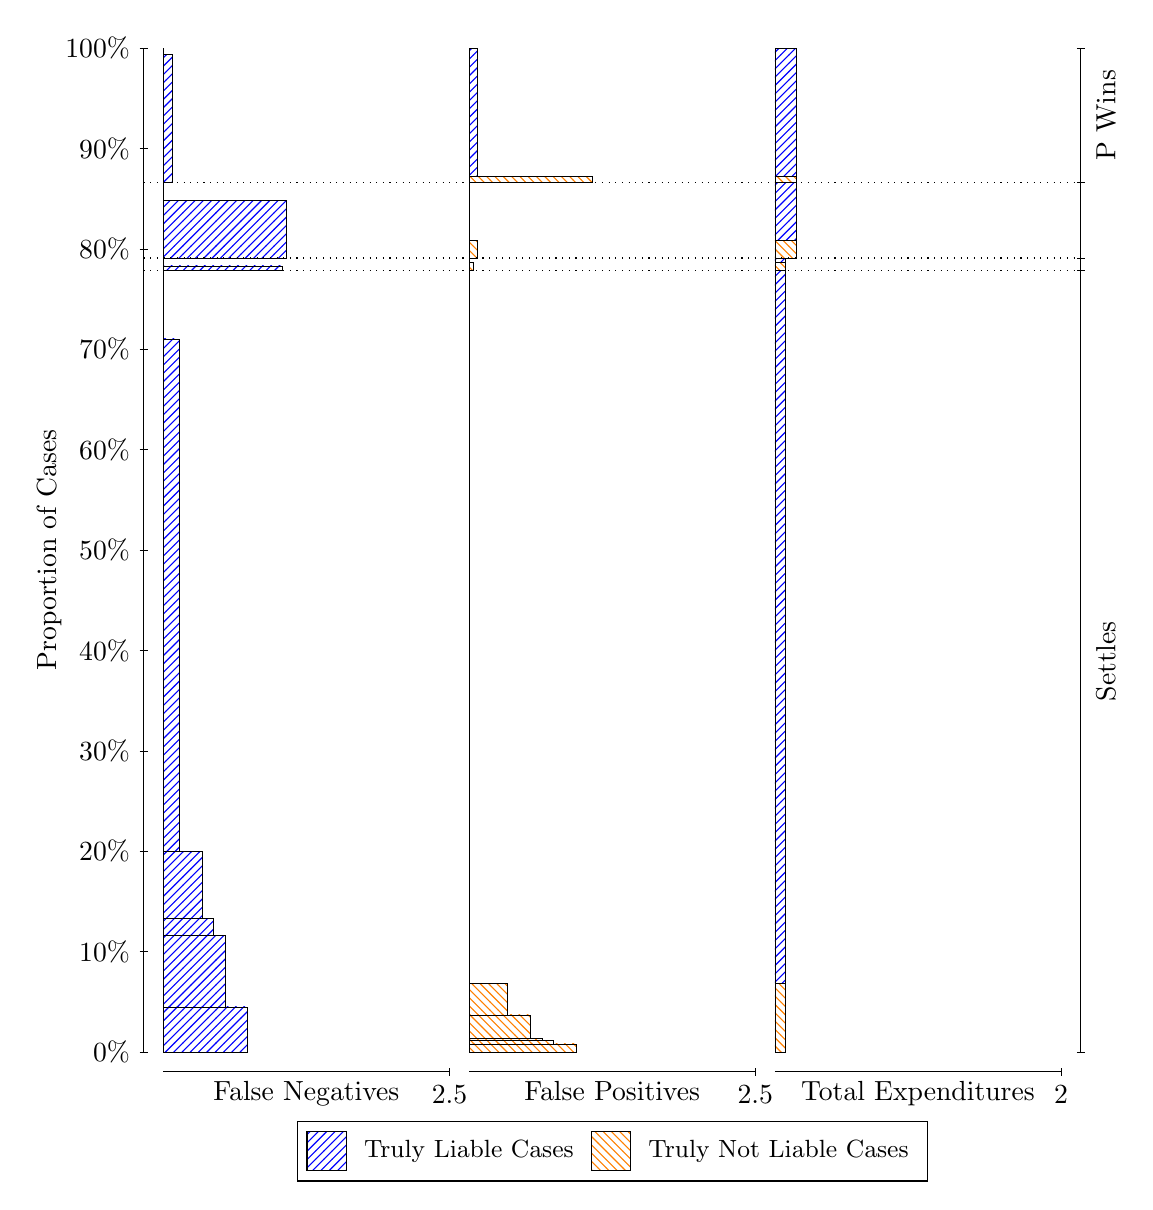
\begin{tikzpicture}
\draw[black, very thin] (1.5,1.75) -- (1.5,14.5);
\node[rotate=90, text=black, anchor=center] at (0.3, 8.125) {Proportion of Cases};
\draw[black, very thin] (1.45,1.75) -- (1.55,1.75);
\node[text=black, anchor=east] at (1.45, 1.75) {0\%};
\draw[black, very thin] (1.45,3.025) -- (1.55,3.025);
\node[text=black, anchor=east] at (1.45, 3.025) {10\%};
\draw[black, very thin] (1.45,4.3) -- (1.55,4.3);
\node[text=black, anchor=east] at (1.45, 4.3) {20\%};
\draw[black, very thin] (1.45,5.575) -- (1.55,5.575);
\node[text=black, anchor=east] at (1.45, 5.575) {30\%};
\draw[black, very thin] (1.45,6.85) -- (1.55,6.85);
\node[text=black, anchor=east] at (1.45, 6.85) {40\%};
\draw[black, very thin] (1.45,8.125) -- (1.55,8.125);
\node[text=black, anchor=east] at (1.45, 8.125) {50\%};
\draw[black, very thin] (1.45,9.4) -- (1.55,9.4);
\node[text=black, anchor=east] at (1.45, 9.4) {60\%};
\draw[black, very thin] (1.45,10.675) -- (1.55,10.675);
\node[text=black, anchor=east] at (1.45, 10.675) {70\%};
\draw[black, very thin] (1.45,11.95) -- (1.55,11.95);
\node[text=black, anchor=east] at (1.45, 11.95) {80\%};
\draw[black, very thin] (1.45,13.225) -- (1.55,13.225);
\node[text=black, anchor=east] at (1.45, 13.225) {90\%};
\draw[black, very thin] (1.45,14.5) -- (1.55,14.5);
\node[text=black, anchor=east] at (1.45, 14.5) {100\%};

\draw[black, very thin] (13.4,1.75) -- (13.4,14.5);
\draw[black, very thin] (13.35,1.75) -- (13.45,1.75);
\node[anchor=west] at (13.35, 1.75) {};
\draw[black, very thin] (13.35,11.674) -- (13.45,11.674);
\node[anchor=west] at (13.35, 11.674) {};
\draw[black, very thin] (13.35,11.833) -- (13.45,11.833);
\node[anchor=west] at (13.35, 11.833) {};
\draw[black, very thin] (13.35,12.793) -- (13.45,12.793);
\node[anchor=west] at (13.35, 12.793) {};
\draw[black, very thin] (13.35,14.5) -- (13.45,14.5);
\node[anchor=west] at (13.35, 14.5) {};

\draw[black, very thin, pattern color=blue, pattern=north east lines] (1.75,1.75) rectangle (2.8218,2.3217);
\draw[black, very thin, pattern color=blue, pattern=north east lines] (1.75,2.3217) rectangle (2.5312,3.2353);
\draw[black, very thin, pattern color=blue, pattern=north east lines] (1.75,3.2353) rectangle (2.3858,3.4506);
\draw[black, very thin, pattern color=blue, pattern=north east lines] (1.75,3.4506) rectangle (2.2405,4.2985);
\draw[black, very thin, pattern color=blue, pattern=north east lines] (1.75,4.2985) rectangle (1.9498,10.806);
\draw[black, very thin, pattern color=orange, pattern=north west lines] (1.75,10.806) rectangle (1.75,11.674);
\draw[black, very thin, pattern color=blue, pattern=north east lines] (1.75,11.674) rectangle (3.2578,11.734);
\draw[black, very thin, pattern color=orange, pattern=north west lines] (1.75,11.734) rectangle (1.75,11.833);
\draw[black, very thin, pattern color=blue, pattern=north east lines] (1.75,11.833) rectangle (3.3123,12.566);
\draw[black, very thin, pattern color=orange, pattern=north west lines] (1.75,12.566) rectangle (1.75,12.793);
\draw[black, very thin, pattern color=blue, pattern=north east lines] (1.75,12.793) rectangle (1.859,14.419);
\draw[black, very thin, pattern color=orange, pattern=north west lines] (1.75,14.419) rectangle (1.75,14.5);
\draw[black, very thin, pattern color=orange, pattern=north west lines] (5.6333,1.75) rectangle (6.9958,1.8524);
\draw[black, very thin, pattern color=orange, pattern=north west lines] (5.6333,1.8524) rectangle (6.7052,1.901);
\draw[black, very thin, pattern color=orange, pattern=north west lines] (5.6333,1.901) rectangle (6.5598,1.9249);
\draw[black, very thin, pattern color=orange, pattern=north west lines] (5.6333,1.9249) rectangle (6.4145,2.2214);
\draw[black, very thin, pattern color=orange, pattern=north west lines] (5.6333,2.2214) rectangle (6.1238,2.618);
\draw[black, very thin, pattern color=blue, pattern=north east lines] (5.6333,2.618) rectangle (5.6333,11.674);
\draw[black, very thin, pattern color=orange, pattern=north west lines] (5.6333,11.674) rectangle (5.6878,11.773);
\draw[black, very thin, pattern color=blue, pattern=north east lines] (5.6333,11.773) rectangle (5.6333,11.833);
\draw[black, very thin, pattern color=orange, pattern=north west lines] (5.6333,11.833) rectangle (5.7423,12.06);
\draw[black, very thin, pattern color=blue, pattern=north east lines] (5.6333,12.06) rectangle (5.6333,12.793);
\draw[black, very thin, pattern color=orange, pattern=north west lines] (5.6333,12.793) rectangle (7.1957,12.874);
\draw[black, very thin, pattern color=blue, pattern=north east lines] (5.6333,12.874) rectangle (5.7423,14.5);
\draw[black, very thin, pattern color=orange, pattern=north west lines] (9.5167,1.75) rectangle (9.6529,2.618);
\draw[black, very thin, pattern color=blue, pattern=north east lines] (9.5167,2.618) rectangle (9.6529,11.674);
\draw[black, very thin, pattern color=orange, pattern=north west lines] (9.5167,11.674) rectangle (9.6529,11.773);
\draw[black, very thin, pattern color=blue, pattern=north east lines] (9.5167,11.773) rectangle (9.6529,11.833);
\draw[black, very thin, pattern color=orange, pattern=north west lines] (9.5167,11.833) rectangle (9.7892,12.06);
\draw[black, very thin, pattern color=blue, pattern=north east lines] (9.5167,12.06) rectangle (9.7892,12.793);
\draw[black, very thin, pattern color=orange, pattern=north west lines] (9.5167,12.793) rectangle (9.7892,12.874);
\draw[black, very thin, pattern color=blue, pattern=north east lines] (9.5167,12.874) rectangle (9.7892,14.5);
\draw[black, dotted] (1.5,11.674) -- (13.4,11.674);
\draw[black, dotted] (1.5,11.833) -- (13.4,11.833);
\draw[black, dotted] (1.5,12.793) -- (13.4,12.793);
\draw[black, very thin] (1.75,1.5) -- (5.3833,1.5);
\node[text=black, anchor=north] at (3.5667, 1.5) {False Negatives};
\draw[black, very thin] (5.3833,1.45) -- (5.3833,1.55);
\node[text=black, anchor=north] at (5.3833, 1.45) {2.5};

\draw[black, very thin] (5.6333,1.5) -- (9.2667,1.5);
\node[text=black, anchor=north] at (7.45, 1.5) {False Positives};
\draw[black, very thin] (9.2667,1.45) -- (9.2667,1.55);
\node[text=black, anchor=north] at (9.2667, 1.45) {2.5};

\draw[black, very thin] (9.5167,1.5) -- (13.15,1.5);
\node[text=black, anchor=north] at (11.333, 1.5) {Total Expenditures};
\draw[black, very thin] (13.15,1.45) -- (13.15,1.55);
\node[text=black, anchor=north] at (13.15, 1.45) {2};

\node[text=black, centered, rotate=90] at (13.72, 6.7119) {Settles};


\node[text=black, centered, rotate=90] at (13.72, 13.646) {P Wins};

\draw (7.449999999999999,1.5) node[draw=none] (baseCoordinate) {};
\begin{scope}[align=center]
        \matrix[scale=0.5, draw=black, below=0.5cm of baseCoordinate, nodes={draw}, column sep=0.1cm]{
            \node[rectangle, draw, minimum width=0.5cm, minimum height=0.5cm, pattern color=blue, pattern=north east lines] {}; &
            \node[draw=none, font=\small, text=black] (B) {Truly Liable Cases}; &
            \node[rectangle, draw, minimum width=0.5cm, minimum height=0.5cm, pattern color=orange, pattern=north west lines] {}; &
            \node[draw=none, font=\small, text=black] (B) {Truly Not Liable Cases}; \\
            };
\end{scope}

\end{tikzpicture}
\end{document}